\documentclass{standalone}
\usepackage{tikz}
\usepackage{ctex,siunitx}
\setCJKmainfont{Noto Serif CJK SC}
\usepackage{tkz-euclide}
\usepackage{amsmath}
\usetikzlibrary{patterns, calc,3d}
\usetikzlibrary {decorations.pathmorphing,decorations.pathreplacing,decorations.shapes}
\tikzset{label style/.append style={font=\small}}
\begin{document}
\small
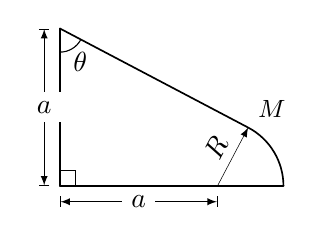
\begin{tikzpicture}[>=latex,scale=1.0]
  \tkzDefPoints{0/0/O,2/0/A,0/2/B,3.8/0/C}
  \tkzDefPointsBy[projection=onto B--C](A){M}
  \tkzInterLC(O,C)(A,M)\tkzGetPoints{D'}{D}
  \tkzDrawArc[semithick](A,D)(M)
  \tkzDrawSegments[semithick](M,B B,O O,D)
  \tkzLabelPoints[above right](M)
  \tkzMarkAngle[size=0.3](O,B,M)
  \tkzLabelAngle[pos=0.5](O,B,M){$\theta$}
  \draw[very thin,->](A)--(M)node[midway,sloped,above]{$R$};
  \tkzMarkRightAngle[size=0.2](C,O,B)
  \draw[very thin,|<->|](0,-0.2)--(2,-0.2)node[midway,fill=white]{$a$};
  \draw[very thin,|<->|](-0.2,0)--(-0.2,2)node[midway,fill=white]{$a$};
\end{tikzpicture}
\end{document}